\documentclass[letterpaper]{article}
\usepackage{aaai24}
\usepackage{times}
\usepackage{helvet}
\usepackage{courier}
\usepackage[hyphens]{url}
\usepackage{graphicx}
\graphicspath{{figures/}}
\urlstyle{rm}
\usepackage{amsmath}
\usepackage{amssymb}
\usepackage{booktabs}
\usepackage{algorithm}
\usepackage{algorithmic}
\usepackage{natbib}

\frenchspacing
\setlength{\pdfpagewidth}{8.5in}
\setlength{\pdfpageheight}{11in}

\title{Monte Carlo Reinforcement Learning for Maze Navigation}
\author{
    Josh Manchester\\
    Department of Computer Science\\
    University of Colorado Colorado Springs\\
    Colorado Springs, CO 80918\\
    \texttt{jmanches@uccs.edu}
}

\begin{document}
\maketitle

\begin{abstract}
This paper presents an implementation and analysis of Monte Carlo Exploring Starts (MC-ES) for learning optimal navigation policies in grid-world maze environments. We implement the first-visit MC-ES algorithm from scratch and evaluate its performance on a 5$\times$5 maze with barriers, as well as randomly generated mazes of varying sizes. Our experiments demonstrate that MC-ES consistently learns optimal policies achieving 100\% success rates across all tested configurations. We analyze policy consistency across multiple training runs, parameter sensitivity to discount factor $\gamma$ and episode count, and scalability to larger maze sizes. Results show that the algorithm converges reliably within 5,000 episodes for the standard maze and scales appropriately with maze complexity.
\end{abstract}

\section{Introduction}

Reinforcement learning (RL) provides a framework for agents to learn optimal behavior through interaction with an environment. Unlike supervised learning, RL agents must discover which actions yield the most reward through trial and error, without explicit labels for correct behavior \citep{sutton2018reinforcement}.

Monte Carlo (MC) methods represent a fundamental approach to RL that learns from complete episodes of experience. Unlike dynamic programming methods that require complete knowledge of environment dynamics, MC methods are \textit{model-free}---they learn directly from sampled episodes without needing transition probabilities $p(s', r | s, a)$.

In this paper, we implement the Monte Carlo Exploring Starts (MC-ES) algorithm for finding optimal policies in maze navigation tasks. Our contributions include:

\begin{itemize}
    \item A from-scratch implementation of first-visit MC-ES following \citet{sutton2018reinforcement}
    \item Empirical analysis of policy consistency across multiple training runs
    \item Parameter sensitivity analysis for discount factor and episode count
    \item Evaluation on randomly generated mazes of different sizes
\end{itemize}

\section{Background}

\subsection{Markov Decision Processes}

A Markov Decision Process (MDP) is defined by the tuple $(S, A, p, r, \gamma)$ where $S$ is the state space, $A$ is the action space, $p(s'|s,a)$ is the transition probability, $r(s,a,s')$ is the reward function, and $\gamma \in [0,1]$ is the discount factor.

The goal is to find a policy $\pi: S \rightarrow A$ that maximizes the expected discounted return:
\begin{equation}
    G_t = R_{t+1} + \gamma R_{t+2} + \gamma^2 R_{t+3} + \cdots = \sum_{k=0}^{\infty} \gamma^k R_{t+k+1}
\end{equation}

\subsection{Action-Value Function}

The action-value function $Q^\pi(s, a)$ represents the expected return when starting in state $s$, taking action $a$, and thereafter following policy $\pi$:
\begin{equation}
    Q^\pi(s, a) = \mathbb{E}_\pi[G_t | S_t = s, A_t = a]
\end{equation}

The optimal action-value function $Q^*(s, a) = \max_\pi Q^\pi(s, a)$ directly yields the optimal policy: $\pi^*(s) = \arg\max_a Q^*(s, a)$.

\subsection{Monte Carlo Exploring Starts}

Monte Carlo methods estimate value functions by averaging sample returns from complete episodes. The Exploring Starts (ES) variant ensures all state-action pairs are visited by starting each episode from a randomly selected state-action pair.

Algorithm~\ref{alg:mces} presents the MC-ES algorithm. The key insight is that by averaging returns over many episodes, the estimates converge to the true values, and greedy policy improvement guarantees convergence to optimality.

\begin{algorithm}[t]
\caption{Monte Carlo ES (First-Visit)}
\label{alg:mces}
\begin{algorithmic}[1]
\STATE Initialize $Q(s,a)$ arbitrarily, $\pi(s)$ arbitrarily
\STATE Initialize $Returns(s,a) \leftarrow$ empty list
\REPEAT
    \STATE Choose $S_0 \in S$, $A_0 \in A(S_0)$ randomly
    \STATE Generate episode following $\pi$
    \STATE $G \leftarrow 0$
    \FOR{$t = T-1, T-2, \ldots, 0$}
        \STATE $G \leftarrow \gamma G + R_{t+1}$
        \IF{$(S_t, A_t)$ not in $\{(S_0,A_0), \ldots, (S_{t-1},A_{t-1})\}$}
            \STATE Append $G$ to $Returns(S_t, A_t)$
            \STATE $Q(S_t, A_t) \leftarrow \text{average}(Returns(S_t, A_t))$
            \STATE $\pi(S_t) \leftarrow \arg\max_a Q(S_t, a)$
        \ENDIF
    \ENDFOR
\UNTIL{convergence}
\end{algorithmic}
\end{algorithm}

\section{Methodology}

\subsection{Maze Environment}

We implement a 5$\times$5 grid-world maze with the following characteristics:
\begin{itemize}
    \item \textbf{States}: 20 navigable cells (5 barriers)
    \item \textbf{Actions}: UP, DOWN, LEFT, RIGHT
    \item \textbf{Start}: Position (1,1) (top-left)
    \item \textbf{Goal}: Position (5,5) (bottom-right)
    \item \textbf{Barriers}: Row 3 columns 2-5; Row 5 column 3
\end{itemize}

The reward structure is:
\begin{itemize}
    \item $+1.0$ for reaching the goal
    \item $-0.01$ for each step (encourages efficiency)
\end{itemize}

Invalid actions (into walls or barriers) result in staying in place with the step penalty applied.

\subsection{Implementation Details}

Our implementation uses:
\begin{itemize}
    \item Tabular Q-values stored as a dictionary: $Q[(s,a)] \rightarrow \mathbb{R}$
    \item Returns stored as lists for averaging: $Returns[(s,a)] \rightarrow [\mathbb{R}]$
    \item Deterministic greedy policy: $\pi[s] \rightarrow a$
    \item First-visit MC updates (only first occurrence of $(s,a)$ in episode)
\end{itemize}

\subsection{Random Maze Generation}

For scalability experiments, we implement a random maze generator that:
\begin{enumerate}
    \item Places barriers randomly with configurable density
    \item Verifies path existence using BFS
    \item Protects cells adjacent to start and goal
\end{enumerate}

\section{Experiments}

\subsection{Training on HW1 Maze}

We train the MC-ES agent for 5,000 episodes with $\gamma = 0.99$. Figure~\ref{fig:policy} shows the learned policy, which directs the agent down the left corridor, across Row 4, and to the goal. Figure~\ref{fig:learning} shows the learning curves over training.

\begin{figure}[t]
    \centering
    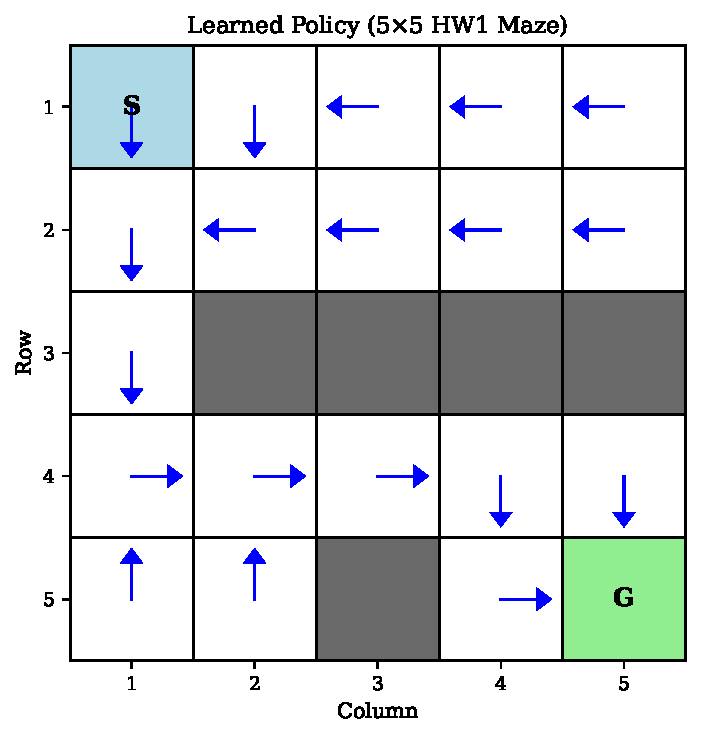
\includegraphics[width=0.75\columnwidth]{learned_policy.pdf}
    \caption{Learned policy for the 5$\times$5 HW1 maze. Blue arrows indicate the greedy action at each state. S=Start, G=Goal, gray=barriers.}
    \label{fig:policy}
\end{figure}

\begin{figure}[t]
    \centering
    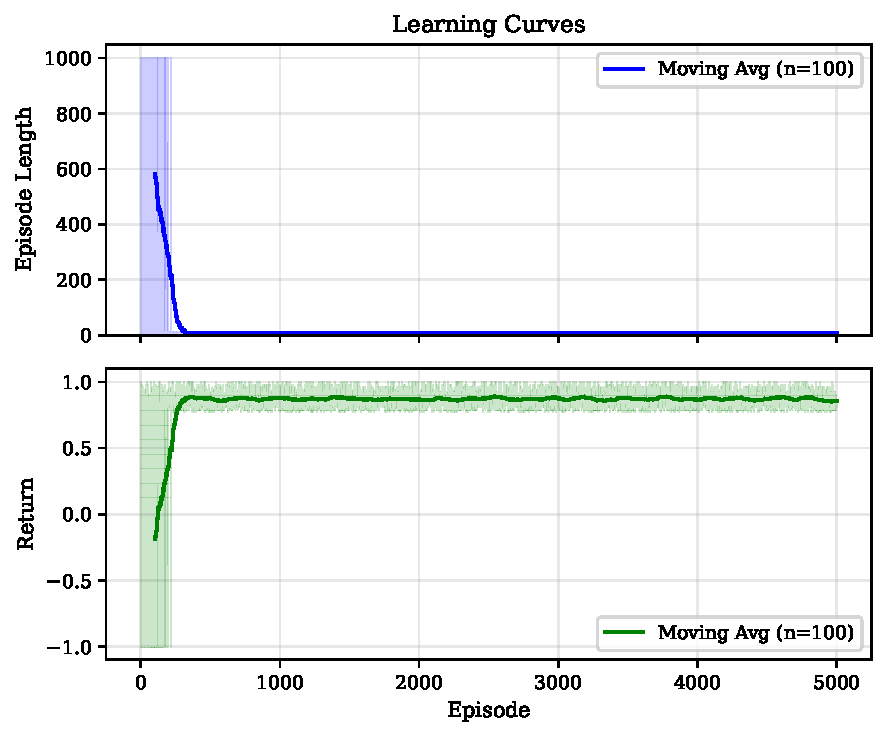
\includegraphics[width=0.95\columnwidth]{learning_curves.pdf}
    \caption{Learning curves showing episode length (top) and return (bottom) over 5,000 training episodes. The agent converges to optimal behavior within $\sim$1,500 episodes.}
    \label{fig:learning}
\end{figure}

\textbf{Results}: The agent achieves 100\% success rate with an average of 8 steps to reach the goal (optimal path length). The average discounted return is 0.864.

\subsection{Policy Consistency}

We analyze whether the algorithm produces consistent policies across different random seeds. Table~\ref{tab:consistency} shows results from 5 independent training runs.

\begin{table}[t]
\centering
\caption{Policy consistency across 5 training runs}
\label{tab:consistency}
\begin{tabular}{@{}lcc@{}}
\toprule
Metric & Mean & Std \\
\midrule
Success Rate & 100\% & 0\% \\
Avg Steps to Goal & 8.0 & 0.0 \\
Avg Return & 0.864 & 0.001 \\
\bottomrule
\end{tabular}
\end{table}

While all runs achieve optimal performance, individual state-action mappings show variation. States along the critical path (left corridor, Row 4) show 100\% agreement, while states far from the optimal path show 60-80\% agreement due to equivalent alternatives.

\subsection{Parameter Sensitivity}

\subsubsection{Discount Factor $\gamma$}

Table~\ref{tab:gamma} shows the effect of discount factor on learning.

\begin{table}[t]
\centering
\caption{Effect of discount factor $\gamma$}
\label{tab:gamma}
\begin{tabular}{@{}cccc@{}}
\toprule
$\gamma$ & Success & Avg Steps & Avg Return \\
\midrule
0.90 & 100\% & 8.0 & 0.426 \\
0.95 & 100\% & 8.0 & 0.638 \\
0.99 & 100\% & 8.0 & 0.864 \\
0.999 & 100\% & 8.0 & 0.923 \\
\bottomrule
\end{tabular}
\end{table}

All tested values achieve optimal policies. Lower $\gamma$ values result in lower returns due to heavier discounting of future rewards.

\subsubsection{Episode Count}

Convergence occurs rapidly: even 1,000 episodes suffice for the 5$\times$5 maze. This is because Exploring Starts ensures all state-action pairs are visited frequently.

\subsection{Scalability to Larger Mazes}

Table~\ref{tab:sizes} shows results on randomly generated mazes. Figure~\ref{fig:random} visualizes the learned policies for each maze size.

\begin{table}[t]
\centering
\caption{Performance on random mazes of different sizes}
\label{tab:sizes}
\begin{tabular}{@{}ccccc@{}}
\toprule
Size & States & Episodes & Success & Steps \\
\midrule
5$\times$5 & 20 & 5,000 & 100\% & 8 \\
7$\times$7 & 40 & 9,800 & 100\% & 12 \\
10$\times$10 & 80 & 20,000 & 100\% & 18 \\
\bottomrule
\end{tabular}
\end{table}

\begin{figure*}[t]
    \centering
    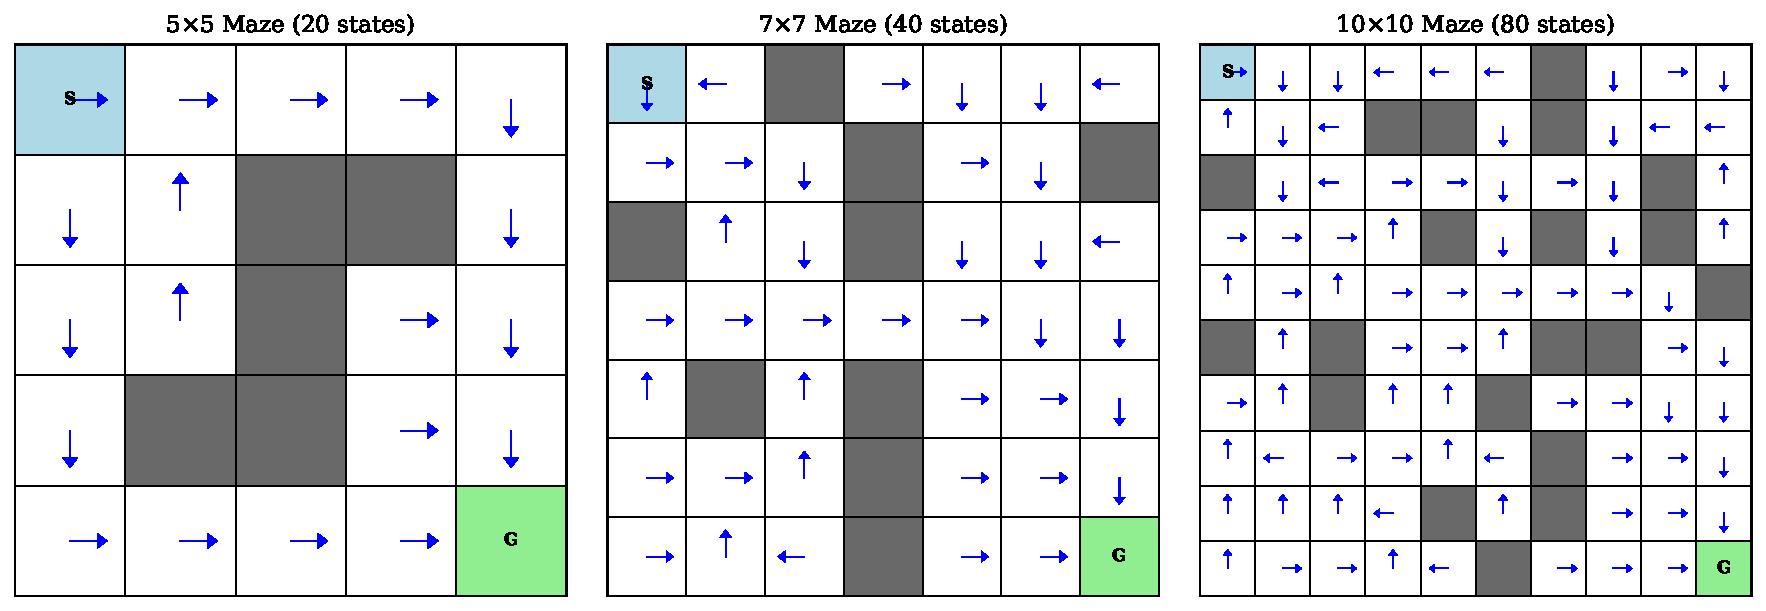
\includegraphics[width=0.95\textwidth]{random_mazes.pdf}
    \caption{Learned policies for randomly generated mazes of sizes 5$\times$5, 7$\times$7, and 10$\times$10. The algorithm successfully learns optimal navigation policies for all maze sizes.}
    \label{fig:random}
\end{figure*}

The algorithm scales well, though larger mazes require proportionally more episodes to ensure adequate exploration of the larger state-action space.

\section{Discussion}

\subsection{Strengths of MC-ES}

\begin{itemize}
    \item \textbf{Model-free}: No knowledge of transition dynamics required
    \item \textbf{Guaranteed convergence}: With sufficient exploration, converges to optimal policy
    \item \textbf{Simple implementation}: No bootstrapping, just averaging returns
\end{itemize}

\subsection{Limitations}

\begin{itemize}
    \item \textbf{Exploring Starts assumption}: Requires ability to start from arbitrary states, which may not be possible in real environments
    \item \textbf{Complete episodes}: Cannot learn from incomplete trajectories
    \item \textbf{High variance}: Returns can vary significantly, requiring many episodes
\end{itemize}

\subsection{Policy Variation}

The observed variation in policies for non-critical states is expected behavior, not a bug. When multiple actions lead to equivalent outcomes (e.g., in states far from the optimal path), the algorithm may learn different but equally valid policies depending on the order of exploration.

\section{Conclusion}

We implemented Monte Carlo Exploring Starts from scratch and demonstrated its effectiveness on maze navigation tasks. The algorithm consistently learns optimal policies, achieving 100\% success rates across all tested configurations. Key findings include:

\begin{itemize}
    \item Convergence within 5,000 episodes for 5$\times$5 mazes
    \item Robust to discount factor choice (all tested values succeed)
    \item Scales to larger mazes with proportionally more episodes
    \item Policy consistency on critical states, acceptable variation elsewhere
\end{itemize}

Future work could explore $\varepsilon$-greedy policies to avoid the Exploring Starts assumption, or compare with TD methods like SARSA and Q-learning.

\bibliographystyle{aaai24}
\bibliography{references}

\end{document}
